\documentclass[a4paper, 12pt]{article} % тип документа

%%%Библиотеки
	%\usepackage[warn]{mathtext}	
	\usepackage[T2A]{fontenc}   %Кодировка
	\usepackage[utf8]{inputenc} %Кодировка исходного текста
	\usepackage[english, russian]{babel} %Локализация и переносы
	\usepackage{caption}
	\usepackage{listings}
	\usepackage{amsmath, amsfonts, amssymb, amsthm, mathtools}
	\usepackage[warn]{mathtext}
	\usepackage[mathscr]{eucal}
	\usepackage{wasysym}
	\usepackage{graphicx} %Вставка картинок правильная
	\DeclareGraphicsExtensions{.pdf,.png,.jpg}
	\graphicspath{ {images/} }
	
	\setlength{\parskip}{0.5cm}
	
	\usepackage{pgfplots}
	\usepackage{indentfirst}
	\usepackage{float}    %Плавающие картинки
	\usepackage{wrapfig}  %Обтекание фигур (таблиц, картинок и прочего)
	\usepackage{fancyhdr} %Загрузим пакет
	\usepackage{lscape}
	\usepackage{xcolor}
	\usepackage[normalem]{ulem}
	\usepackage{wasysym}
	\usepackage{subfig}
	\usepackage{graphicx}
	
	\usepackage{titlesec}
	\titlelabel{\thetitle.\quad}

	\usepackage{hyperref}
	\newenvironment{comment}{}{}

%%%Конец библиотек

%%%Настройка ссылок
%%%	\hypersetup
%%%	{
%%%		colorlinks = true,
%%%		linkcolor  = blue,
%%%		filecolor  = magenta,
%%%		urlcolor   = blue
%%%	}
%%%Конец настройки ссылок


%%%Настройка колонтитулы
    \pagestyle{fancy}
    \fancyhead{}
    \fancyhead[L]{1.1.1}
    \fancyhead[R]{Засимов Георгий, группа Б01-109}
    \fancyfoot[C]{\thepage}
%%%конец настройки колонтитулы



\begin{document}
                        %%%%Начало документа%%%%


%%%Начало титульника
\begin{titlepage}

    \newpage
    \begin{center}
        \normalsize Московский физико-технический институт \\(национальный исследовательский университет)
    \end{center}

    \vspace{6em}

    \begin{center}
        \Large Лабораторная работа по общему курсу физики\\
    \end{center}

    \vspace{1em}

    \begin{center}
        \Large \textbf{1.1.1. Определение систематических и случайных погрешностей при измерении удельного сопротивления нихромовой проволки}
    \end{center}

    \vspace{2em}

    \begin{center}
        \large Засимов Георгий Алексеевич \\
        Группа Б01-109
    \end{center}

    \vspace{\fill}

    \begin{center}
    Долгопрудный \\2021
    \end{center}
    
\end{titlepage}
%%%Конец Титульника


%%%%Настройка оглавления и нумерации страниц
%%%    \thispagestyle{empty}
%%%    \newpage
%%%    \tableofcontents
%%%    \newpage
%%%    \setcounter{page}{1}
%%%%Настройка оглавления и нумерации страниц

\section*{1. Аннотация}

\textbf{Цель работы:} измерить удельное сопротивление проволоки и вычислить систематические и случайные погрешности при использовании таких измерительных приборов, как линейка, штангенциркуль, микрометр, амперметр, вольтметр и мост постоянного тока.\\

\textbf{Используемое оборудование:} линейка, штангенциркуль, микрометр, отрезок проволоки из нихрома, амперметр, вольтметр, источник ЭДС, мост постоянного тока, реостат, ключ.\\

\textbf{Используются следующие методы измерений сопротивления:} 

1) Определение углового коэффициента наклона зависимости напряжения на проволоке от тока через неё, измеряемых с помощью аналоговых и цифровых вольтметров и амперметров.

2) Измерение с помощью моста постоянного тока. Геометрические размеры образца измеряются с помощью линейки, штангенциркуля и микрометра. Детально исследуется систематические и случайные погрешности проводимых измерений.

В данной работе мы используем оба метода и сравниваем их.\\


\section*{2. Теоретические сведения}

Удельное сопротивленеи проволоки круглого сечения, изготовленного из однородного материала и имеющей всюду одинаковую толщину, может быть определено по формуле
\[\rho = \frac{R_{\text{пр}}}{L} \frac{\pi d^2}{4}\]

В этой формуле $R$ -- сопротивление измеряемого отрезка проволоки, $d$ -- диаметр проволоки, $L$ -- длина отрезка проволоки.

Так как диаметр проволоки флуктуирует в зависимости от места измерения и толщины, необходимо найти среднее значение толщины по всей длине проволоки. Также необходимо учесть погрешность измеренной средней толщины при подсчёте погрешности удельного сопротивления проволоки.

Сопротивление проволоки можно искать с помощью двух различных (очень схожих) электрических схем:
\begin{center}
    {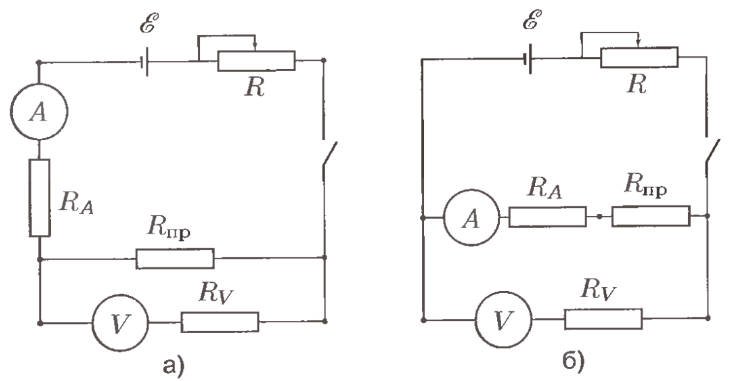
\includegraphics[width=11cm]{1}}
\end{center}

На данных схемах $R_V$ и $R_A$ -- сопротивления вольтметра и амперметра соответственно, а $R$ -- сопротивление реостата.

Для схемы a) имеем:
\[R_{\text{пр1}} = \frac{V_a}{I_a} = R_{\text{пр}} \frac{R_V}{R_V + R_{\text{пр}}} \]

Здесь $R_{\text{пр1}}$ -- измеренное сопротивление проволоки по закону Ома без учёта конечности сопротивления вольметра.

Для схемы б) имеем:
\[R_{\text{пр2}} = \frac{V_{\text{б}}}{I_{\text{б}}} = R_{\text{пр}} + R_A\]

Здесь $R_{\text{пр2}}$ -- измеренное сопротивление проволоки по закону Ома без учёта того, что у амперметра есть сопротивление.

Преобразуем оба выражения:
\[R_{\text{пр}} = R_{\text{пр1}} \frac{R_V}{R_V - R_{\text{пр1}}} = \frac{R_{\text{пр1}}}{1 - (R_{\text{пр1}})/(R_V)} \cong R_{\text{пр1}} (1 + \frac{R_{\text{пр1}}}{R_V})\]

\[R_{\text{пр}} = R_{\text{пр1}} (1 - \frac{R_A}{R_{\text{пр2}}})\]

Естественно, использовтаь надо то выражение, которое даёт меньшую поправку на сопротивление.\\

\section*{3. Оборудование и инструментальные погрешности}


\textbf{Линейка:} $\vartriangle_{лин} = 0,5$ мм (по цене деления). 
%%При определении положений контактов имеется дополнительная погрешность, которая может быть оценена как  $\vartriangle_{лин} = \pm2$ мм.\\
\textbf{Штангенциркуль:} $\vartriangle_{шт} = 0,1$ мм (маркировка производителя).\\
\textbf{Микрометр:} $\vartriangle_{мкм} = 0,01$ мм (маркировка производителя).\\
\textbf{Вольтметр:} погрешность измерения вольтметра вычисляется согласно паспорту устройства для используемого напряжения 5В по формуле: $\vartriangle_{вм} = \pm(0,0003 X + 4 k)$ мВ , где X -- полученное значение напряжения, k -- порядок полученного измерения.\\
\textbf{Амперметр:} при измерниях в диапазоне 20 мА до 300 мА погрешность амперметра составила 0,5\%. \\


%%%В диапазоне измерения R от 1 до 10 Ом относительная поправка $\frac{R'}{R_{V}}$ к сопротивлению согласно формуле \eqref{сопр образца} составляет от 0,01\% (при R = 1 Oм и $R_{V}$ 10 кОм) до 0,2\% (при R 10 Ом и
%%%$R_{V}$ кОм). Следовательно, данная поправка заведомо меньше погрешности измерений (0,5\% для вольтметра), поэтому примем далее, что неидеальность вольтметра не оказывает влияния на измерение сопротивления:   $R \approx R'$\\\\\\

\textbf{Мост постоянного тока Р4833:}\\
Класс точности: 0,1\\
Разрядность магазина сопротивлений: 5 ед.\\
Используемый диапазон измерений: 10-4 - 10 Ом (для множителя $N = 10^2$).\\
Погрешность измерений в используемом диапазоне: ±0,010 Ом.\\

\section*{4. Результаты измерений и обработка данных}
\subsection*{4.1 \textit{Измерение диаметра d проволоки}}


Измерения проводились штангенциркулем и микрометром многократно на разных участках
проволоки. При измерении штангенциркулем и микрометром выявлен разброс в показаниях, (см. табл. 1.)\\




Среднее значение диаметра при измерении штангенциркулем: $\overline{d} = \frac{\sum d_{i}}{N} = 0,375$. И микрометром: $\overline{d} = \frac{\sum d_{i}}{N} = 0,361$ мм. 


\begin{flushright}
{\scriptsize \textbf{Таблица 1.}\\Измерения диаметра проволоки штангенциркулем и микрометром.}
\end{flushright} 


\begin{table}[h!]
\begin{tabular}{|l|l|l|l|l|l|l|l|l|}
\hline
N измерения          & 1    & 2    & 3    & 4    & 5    & 6    & 7    & 8    \\ \hline
Штангенциркуль d, мм & 0,4  & 0,3  & 0,4  & 0,4  & 0,4  & 0,3  & 0,4  & 0,4  \\ \hline
Микрометр d, мм      & 0,36 & 0,36 & 0,35 & 0,36 & 0,36 & 0,36 & 0,37 & 0,37 \\ \hline
\end{tabular}
\end{table}


Стандартное отклонение для измерения штангенциркулем(в мм):
\begin{equation}
    \sigma_{d} = \sqrt{\frac{1}{N-1}\sum (d_{i}-\overline{d})^2} = 0,037
\end{equation}


И микрометром (в мм):
\begin{equation}
    \sigma_{d} = \sqrt{\frac{1}{N-1}\sum (d_{i}-\overline{d})^2} = 0,005
\end{equation}


Случайная погрешность среднего для штангенциркуля (в мм):
\begin{equation}
    \sigma_{\overline{d}} = \frac{\sigma_{d}}{\sqrt{N}} = 0,016
\end{equation}


И для микрометра (в мм):
\begin{equation}
    \sigma_{\overline{d}} = \frac{\sigma_{d}}{\sqrt{N}} = 0,0001
\end{equation}


С учётом инструментальной погрешности $\Delta _{мкм} = 0,01$ мм и $\Delta _{штц} = 0,1$ мм погрешность измерения диаметра
может быть вычислена для штангенциркуля так (в мм):
\begin{equation}
    \sigma{_{\overline{d}}} = \sqrt{\sigma{_{\overline{d}}}^2 + \Delta_{мкм}^2} \approx 0,101
\end{equation}


И для микрометра (в мм):
\begin{equation}
    \sigma {_{\overline{d}}} = \sqrt{\sigma{_{\overline{d}}}^2 + \Delta_{штц}^2} \approx 0,01
\end{equation}


\textit{Окончательные результаты измерения диаметра проволоки:}


Микрометром: $d = 0,361 \pm 0,01$мм $(\varepsilon_{d} = 2,8\%)$\\
Штангенциркулем: $d = 0,375 \pm 0,1$ мм

\subsection*{4.2 \textit{Изменение сопротивления проволоки }}

Результаты измерений зависимостей показаний вольтметра $U_{B}$ от показаний амперметра $I_{A}$ в схеме рис. 1 при разных длинах l образца представлены в табл. 2. Соответствующие графики зависимостей изображены на рис. 2. (Поскольку цена деления нашего амперметра равняется 5 мА, а измерения записывались в делениях, в таблице для удобства приведены значения,уже переведённые в мА.)

По графику убеждаемся, что экспериментальные данные с хорошей точностью (в пределах инструментальных погрешностей опыта) ложатся на теоретическую прямую $U = RI$, исходящую из начала координат.

Пользуясь методом наименьших квадратов, строим аппроксимирующие прямые $U_{B} = \overline{R}I_{A}$, определяя их угловой коэффициент по формуле


\[\overline{R} = \frac{\langle UI \rangle}{\langle I^2 \rangle}\]


Случайную погрешность определения углового коэффициента вычисляем как
\[\sigma{^{сл}}{_{\overline{d}}} = \sqrt{\frac{1}{n-1}\left(\frac{U^2}{I^2} - \overline{R}^2\right)}.\]


(где n = 11 – число точек на графике).


Оценим возможную систематическую погрешность, обусловленную инструментальными
погрешностями приборов. Предполагая, что при всех измерениях относительная погрешность приборов одинакова, оценим погрешность вычисления частного R = U/I при максимальных
значениях U и I:
\[\Delta{_{R}} \sim R \sqrt{\left(\frac{\Delta{_{U}}}{U_{max}}\right)^2 + \left( \frac{\Delta{_{l}}}{l_{max}}\right)^2}\]


\begin{flushleft}
{\scriptsize \textbf{Таблица 2.}\\Зависимость $U_{B}$ от $I_{A}$ для разных длин проволоки l.}
\end{flushleft}




\begin{table}[h]
\centering
\begin{tabular}{|l|l|l|l|l|l|l|}
\hline
      & \multicolumn{6}{c|}{l = (50,0 +- 0,2 ) см}          \\ \hline
$U_B$, мВ & 1066,6 & 1164,6 & 1351,5 & 1637,2 & 2006,5 & 3282   \\ \hline
$I_A$, мА & 220    & 235    & 275    & 330    & 400    & 640    \\ \hline
      & \multicolumn{6}{c|}{l = (30,0 +- 0,2 ) см}          \\ \hline
$U_B$, мВ & 663    & 771    & 934,6  & 1106,6 & 1550,1 & 2274,7 \\ \hline
$I_A$, мА & 225    & 260    & 315    & 370    & 470    & 740    \\ \hline
      & \multicolumn{6}{c|}{l = (20,0 +- 0,2 ) см}          \\ \hline
$U_B$, мВ & 439,5  & 499,1  & 555,6  & 695,5  & 810,5  & 1180   \\ \hline
$I_A$, мА & 225    & 255    & 280    & 350    & 405    & 580    \\ \hline
\end{tabular}
\end{table}


\begin{table}[h]
\centering
\begin{tabular}{|l|l|l|l|l|l|l|}
\hline
      & \multicolumn{6}{c|}{l = (50,0 +- 0,2 ) см}          \\ \hline
$U_B$, мВ & 2789,2 & 2346,8 & 1827,6 & 1503,2 & 1234,5 & 1133,2 \\ \hline
$I_A$, мА & 550    & 465    & 365    & 305    & 250    & 230    \\ \hline
      & \multicolumn{6}{c|}{l = (30,0 +- 0,2 ) см}          \\ \hline
$U_B$, мВ & 1945,2 & 1678,7 & 1223,1 & 1046,7 & 834,2  & 692,1  \\ \hline
$I_A$, мА & 635    & 505    & 410    & 350    & 280    & 235    \\ \hline
      & \multicolumn{6}{c|}{l = (20,0 +- 0,2 ) см}          \\ \hline
$U_B$, мВ & 180,1  & 826    & 742,1  & 568,1  & 516,4  & 418,6  \\ \hline
$I_A$, мА & 580    & 415    & 365    & 290    & 265    & 215    \\ \hline
\end{tabular}
\end{table}




Полная погрешность измерения R не превосходит значения 


\[\sigma{_{R}} \leq \sqrt{(\sigma_{R})^2 + (\Delta_{R})^2}\]


Результаты сведены в табл. 3. Там же для сравнения приведены результаты измерения R c помощью моста постоянного тока Р4833 с учётом его погрешности.
\begin{flushright}
{\scriptsize \textbf{Таблица 3.}\\Результаты измерения сопротивления проволоки двумя методами.}
\end{flushright}


\begin{table}[h!]
\centering
\begin{tabular}{|l|l|l|l|l|l|}
\hline
l, см & $\overline R$, Ом & $\sigma_R$, Ом & $\Delta_R$, Ом & $\sigma_R$, Ом & $R_{мост}$, Ом                  \\ \hline
50    & 6,261            & 0,062          & 0,017          & 0,064          & 5,371 $\pm$ 0,010 \\ \hline
30    & 3,779            & 0,187          & 0,014          & 0,188          & 3,402 $\pm$ 0,010  \\ \hline
20    & 2,111            & 0,0034         & 0,016          & 0,016          & 2,478 $\pm$ 0,010  \\ \hline
\end{tabular}
\end{table}
Видно, что случайная составляющая измерения сопротивления мала, а основной вклад вносят систематические приборные погрешности. Контрольные измерения с помощью моста дают заниженные результаты, но все отклонения находятся в пределах $\pm 2 \sigma_{R}$.
полн.


\begin{center}
    {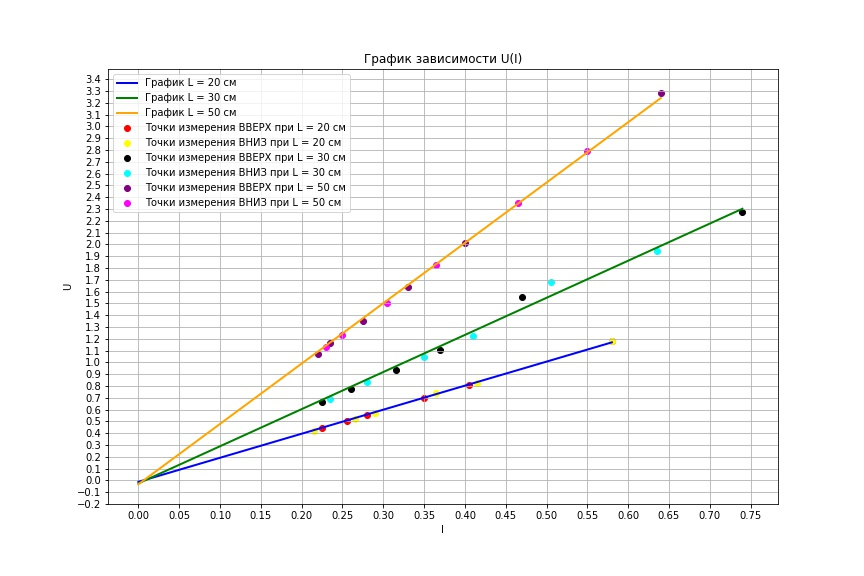
\includegraphics[width=14cm]{schedule}}
\end{center}

Рис. 2. Результаты измерений напряжения $U_B$ в зависимости от тока $I_A$ для проволок разной длины l и их линейная аппроксимация $y=kx$.\\


%%%Не отмечены инструментальные погрешности по вертикальной и горизонтальной осям ввиду их малости ($\sigma_v = 3,8$ мВ, $\sigma_{I}$ - см. п. 2).\


\subsection*{4.3 \textit{Вычисление удельного сопротивления}}




По формуле (1) находим удельное сопротивление материала проволоки, используя значения $\overline{R}$, полученные п. 4.2. Сравнивая относительные величины погрешностей величин, входящих в (1), приходим к выводу, что наибольший вклад в погрешность вносит измерение диаметра проволоки $(2\sigma_{d}/d \sim 6,5\%)$, при этом вкладом остальных измерений можно принебречь: $\sigma_{\rho} \approx \frac{2\sigma_{d}}{d}\rho$. Результаты трёх опытов приведены в таблице ниже.


\begin{table}[h]
\centering
\begin{tabular}{|l|l|}
\hline
N опыта & $\rho, 10^{-6}$ Ом м   \\ \hline
1       & $1,33 \pm 0,08$                         \\ \hline
2       & $1,34 \pm 0,08$                         \\ \hline
3       & $1,12 \pm 0,07$                         \\ \hline
\end{tabular}
\end{table}


Усредняя результаты трёх опытов, окончательно получим:\\


$\underline{\overline{\rho} = (1,25 \pm 0,08)\cdot{10^{-6}}}$ Ом м ($\varepsilon_{\rho} = 6,6\%$)\


\section*{5. Обсуждение результатов и выводы}


В работе получено значение удельного сопротивления образца проволоки из нихромового сплава с точностью 6,6\%. Табличные значения для нихрома лежат в диапазоне $\rho_{табл} = 0,97 .... 1,14\cdot10^{-6}$ Ом м в зависимости от состава. Измеренные значения $\rho = (1,25 \pm 0,08) \cdot 10^{-6}$ Ом м попадают в этот диапазон в пределах трех стандартных отклонений. 


На графике измерения $U_B$ относительно $I_A$ при $l = 30$см наблюдается большое количество значений, которые не принадлежат аппроксимируещей прямой, 2 из которых ярковыражены. Данное отклонение может быть вызвано человеческими ошибками во время измерения. Стоит отметить, что эти отклонения находятся в пределе 3$\sigma$, что соответствует закону Гауссового распределения (в пределах 3$\sigma$ должны находиться 99\% измерений). В таком случае эти отклонения не оказывают существенного влияния на итогоовый результат измерения.\
\\

Использованный в работе метод измерения сопротивлений позволил получить значения R образцов с довольно высокой точностью (0,5\%), которая ограничивалась в основном погрешностью аналогового вольтметра. Величина случайной погрешности $\sigma_{R}$, найденная в п. 4.2., показывает, что использование более совершенных измерительных приборов позволило бы довести точность измерения по данной методике до 0,1–0,2\% (при неизменном количестве измерений), что сопоставимо с точностью измерений с помощью мостовой схемы.


Точность измерения удельного сопротивления $\rho$ существенно ограничивается измерением диаметра проволоки. Поскольку случайная ошибка измерения диаметра оказалась меньше цены деления прибора (микрометра), уточнение значения диаметра за счет многократных измерений невозможно. По той же причине не удалось убедиться, является ли проволока однородной по сечению или нет.


\end{document}